The simulation of chemical processes supplies valuable insight into the intricacies of a given system.
To some extend it is also possible to improve given designs by manual alterations and simulation
steps in a form of trial an error procedure. However the results of an approach like that are unlikely
to yield even locally optimal results in an acceptable amount of time. Hence optimization approaches
are employed to attain improved designs.

The models presented in the previous chapters are capable of projecting various continuous and
discrete design decisions. However when synthesizing a process flowsheet, one must take careful
consideration as to the optimization objectives. The most obvious objective would be of
pure monetary nature, where a process is designed to meet a given set of specifications
at minimum cost. An optimization like that can be carried out at steady state. However for
a steady state model it is never ensured, that this steady state can actually be reached
by the process. Furthermore is there no consideration if the desired steady state can be kept for
changing conditions outside the control of the process operator.

In the case that load changes or different operation modes are required, it becomes questionable,
if steady state optimization remains feasible, or if a dynamic approach becomes necessary.

In this chapter different optimization studies will be given. For once different solution approaches
will be applied to the MINLP arising from a steady state simulation. For once the outer approximation
algorithm as implemented in \gproms, and secondly the continuous reformulation strategy as described
in \Secref{sec:opt:theory:continuous}.

The process under consideration is a generic cryogenic air separation process. As a starting point for the
optimization a base case was manually constructed which met certain somewhat arbitrarily chosen,
but reasonable constraints.

    \subsection{Example process}
    \begin{figure}
        \footnotesize
        \center
        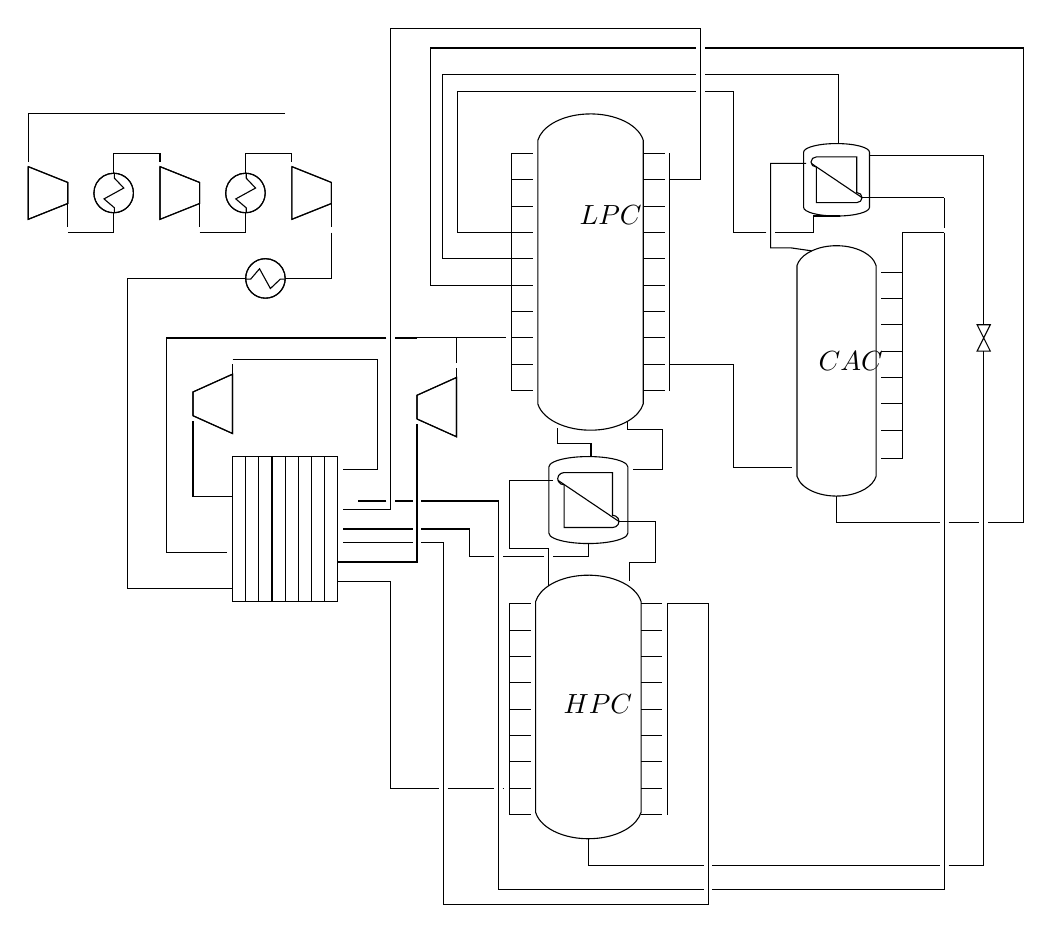
\begin{tikzpicture}[y=0.80pt,x=0.80pt,yscale=-1, inner sep=0pt, outer sep=0pt,scale=0.7]
  \begin{scope}[shift={(555.591,-486.85)}]
      \path[draw] (21.2600,795.1200){[rotate=-180.0] arc(90.001:0.027:21.259800 and 5.613)}
        -- (0.0000,836.2800){[rotate=-180.0] arc(359.973:269.999:21.259800 and
        5.613)}{[rotate=-180.0] arc(270.001:180.027:21.259800 and 5.613)} --
        (42.5200,800.7300){[rotate=-180.0] arc(179.973:89.999:21.259800 and 5.613)} --
        cycle;
    \begin{scope}[shift={(4.77262,-8.61583)}]
      \path[draw] (3.4700,812.3500){[rotate=-180.0] arc(89.984:0.039:3.470990 and
        3.282)}{[rotate=-180.0] arc(359.961:270.016:3.470990 and 3.282)} --
        (3.4700,841.8900) -- (29.5000,841.8900){[rotate=-180.0]
        arc(269.984:180.039:3.470990 and 3.282)}{[rotate=-180.0]
        arc(179.961:90.016:3.470990 and 3.282)} -- (29.5000,812.3500) --
        (3.4700,812.3500) -- cycle;
    \end{scope}
  \end{scope}
  \begin{scope}[shift={(384.094,-348.661)}]
    \path[draw] (0.0000,824.8800){[rotate=-180.0] arc(349.683:190.317:34.574000 and
      20.715)} -- (68.0300,654.8000){[rotate=-180.0] arc(169.683:10.317:34.574000
      and 20.715)} -- (0.0000,824.8800) -- cycle;
    \path[draw] (26.9,709.43) node[above right] (text8791) {$LPC$};
  \end{scope}
  \begin{scope}[shift={(382.677,-85.0394)}]
    \path[draw] (0.0000,824.8800){[rotate=-180.0] arc(349.683:190.317:34.574000 and
      20.715)} -- (68.0300,688.8200){[rotate=-180.0] arc(169.683:10.317:34.574000
      and 20.715)} -- (0.0000,824.8800) -- cycle;
    \path[draw] (18.05,761.05) node[above right] (text8800) {$HPC$};
  \end{scope}
  \begin{scope}[shift={(551.339,-306.142)}]
    \path[draw] (0.0000,829.1300){[rotate=-180.0] arc(349.668:190.332:25.930500 and
      15.537)} -- (51.0200,693.0700){[rotate=-180.0] arc(169.668:10.332:25.930500
      and 15.537)} -- (0.0000,829.1300) -- cycle;
    \path[draw] (14,761.05) node[above right] (text8809) {$CAC$};
  \end{scope}
  \begin{scope}[shift={(187.087,-238.11)}]
    \path[draw] (0.0000,841.8900) -- (68.0300,841.8900) -- (68.0300,748.3500) --
      (0.0000,748.3500) -- (0.0000,841.8900) -- cycle;
    \path[draw] (0.0000,841.8900) -- (68.0300,841.8900) -- (68.0300,748.3500) --
      (0.0000,748.3500) -- (0.0000,841.8900);
    \path[draw] (8.5000,841.8900) -- (8.5000,748.3500);
    \path[draw] (17.0100,841.8900) -- (17.0100,748.3500);
    \path[draw] (25.5100,841.8900) -- (25.5100,748.3500);
    \path[draw] (34.0200,841.8900) -- (34.0200,748.3500);
    \path[draw] (42.5200,841.8900) -- (42.5200,748.3500);
    \path[draw] (51.0200,841.8900) -- (51.0200,748.3500);
    \path[draw] (59.5300,841.8900) -- (59.5300,748.3500);
  \end{scope}
  \begin{scope}[shift={(255.118,-250.866)}]
    \path[draw] (0.0000,841.8900) -- (34.0200,841.8900) -- (34.0200,975.1200) --
      (65.2000,975.1200);
    \path[draw] (70.8700,975.1200) -- (100.6300,975.1200);
    \path[draw] (106.3000,975.1200) -- (107.2800,975.1200);
  \end{scope}
  \begin{scope}[shift={(255.118,-263.622)}]
    \path[draw] (0.0000,841.8900) -- (51.0200,841.8900) -- (51.0200,770.6700);
  \end{scope}
  \begin{scope}[shift={(306.142,1301.1)},xscale=1.000,yscale=-1.000]
    \path[draw] (0.0000,815.1000) -- (0.0000,830.4100) -- (25.5100,841.8900) --
      (25.5100,803.6200) -- (0.0000,815.1000) -- cycle;
    \path[draw] (0.0000,794.0600) -- (0.0000,811.8300);
    \path[draw] (25.5100,841.8900) -- (25.5100,848.1900);
    \path[draw] (0.0000,815.1000) -- (0.0000,830.4100) -- (25.5100,841.8900) --
      (25.5100,803.6200) -- (0.0000,815.1000);
  \end{scope}
  \begin{scope}[shift={(567.726,-464.378)}]
    \path[draw] (-6.9400,841.8900) -- (-20.1700,839.9700) -- (-33.4000,839.9700) --
      (-33.4000,785.4200) -- (-10.5100,785.4200);
  \end{scope}
  \begin{scope}[shift={(306.142,-408.189)}]
    \path[draw] (0.0000,841.8900) -- (-14.1700,841.8900);
    \path[draw] (-19.8400,841.8900) -- (-161.5700,841.8900) -- (-161.5700,980.0800) --
      (-122.3300,980.0800);
  \end{scope}
  \begin{scope}[shift={(452.126,-534.331)}]
    \path[draw] (0.0000,848.9800) -- (13.7400,848.9800);
  \end{scope}
  \begin{scope}[shift={(452.126,-503.15)}]
    \path[draw] (0.0000,834.8000) -- (13.7400,834.8000);
  \end{scope}
  \begin{scope}[shift={(452.126,-486.142)}]
    \path[draw] (0.0000,834.8000) -- (13.7400,834.8000);
  \end{scope}
  \begin{scope}[shift={(452.126,-469.134)}]
    \path[draw] (0.0000,834.8000) -- (13.7400,834.8000);
  \end{scope}
  \begin{scope}[shift={(452.126,-452.126)}]
    \path[draw] (0.0000,834.8000) -- (13.7400,834.8000);
  \end{scope}
  \begin{scope}[shift={(452.126,-435.118)}]
    \path[draw] (0.0000,834.8000) -- (13.7400,834.8000);
  \end{scope}
  \begin{scope}[shift={(452.126,-418.11)}]
    \path[draw] (0.0000,834.8000) -- (13.7400,834.8000);
  \end{scope}
  \begin{scope}[shift={(452.126,-401.102)}]
    \path[draw] (0.0000,834.8000) -- (13.7400,834.8000);
  \end{scope}
  \begin{scope}[shift={(626.457,-348.661)}]
    \path[draw] (-7.0900,841.8900) -- (-7.0900,824.8800);
  \end{scope}
  \begin{scope}[shift={(619.37,-355.748)}]
    \path[draw] (0.0000,848.9800) -- (-13.7400,848.9800);
  \end{scope}
  \begin{scope}[shift={(620.787,1333.7)},rotate=180.0]
  \end{scope}
  \begin{scope}[shift={(619.37,-372.756)}]
    \path[draw] (0.0000,848.9800) -- (-13.7400,848.9800);
  \end{scope}
  \begin{scope}[shift={(620.787,1316.69)},rotate=180.0]
  \end{scope}
  \begin{scope}[shift={(612.283,-365.669)}]
    \path[draw] (7.0900,841.8900) -- (7.0900,824.8800);
  \end{scope}
  \begin{scope}[shift={(619.37,-375.591)}]
    \path[draw] (0.0000,834.8000) -- (-13.7400,834.8000);
  \end{scope}
  \begin{scope}[shift={(620.787,1299.69)},rotate=180.0]
  \end{scope}
  \begin{scope}[shift={(612.283,-382.677)}]
    \path[draw] (7.0900,841.8900) -- (7.0900,824.8800);
  \end{scope}
  \begin{scope}[shift={(619.37,-406.772)}]
    \path[draw] (0.0000,848.9800) -- (-13.7400,848.9800);
  \end{scope}
  \begin{scope}[shift={(620.787,1282.68)},rotate=180.0]
  \end{scope}
  \begin{scope}[shift={(626.457,-399.685)}]
    \path[draw] (-7.0900,841.8900) -- (-7.0900,824.8800);
  \end{scope}
  \begin{scope}[shift={(619.37,-423.78)}]
    \path[draw] (0.0000,848.9800) -- (-13.7400,848.9800);
  \end{scope}
  \begin{scope}[shift={(620.787,1265.67)},rotate=180.0]
  \end{scope}
  \begin{scope}[shift={(612.283,-416.693)}]
    \path[draw] (7.0900,841.8900) -- (7.0900,824.8800);
  \end{scope}
  \begin{scope}[shift={(619.37,-440.787)}]
    \path[draw] (0.0000,848.9800) -- (-13.7400,848.9800);
  \end{scope}
  \begin{scope}[shift={(620.787,1248.66)},rotate=180.0]
  \end{scope}
  \begin{scope}[shift={(626.457,-433.701)}]
    \path[draw] (-7.0900,841.8900) -- (-7.0900,824.8800);
  \end{scope}
  \begin{scope}[shift={(619.37,-457.795)}]
    \path[draw] (0.0000,848.9800) -- (-13.7400,848.9800);
  \end{scope}
  \begin{scope}[shift={(620.787,1231.65)},rotate=180.0]
  \end{scope}
  \begin{scope}[shift={(534.331,-317.48)}]
    \path[draw] (0.0000,834.8000) -- (13.7400,834.8000);
  \end{scope}
  \begin{scope}[shift={(532.913,-323.15)}]
  \end{scope}
  \begin{scope}[shift={(360.0,-527.244)}]
    \path[draw] (7.0900,841.8900) -- (7.0900,858.9000);
  \end{scope}
  \begin{scope}[shift={(367.087,-520.157)}]
    \path[draw] (0.0000,834.8000) -- (13.7400,834.8000);
  \end{scope}
  \begin{scope}[shift={(365.669,-525.827)}]
  \end{scope}
  \begin{scope}[shift={(367.087,-503.15)}]
    \path[draw] (0.0000,834.8000) -- (13.7400,834.8000);
  \end{scope}
  \begin{scope}[shift={(365.669,-508.819)}]
  \end{scope}
  \begin{scope}[shift={(360.0,-510.236)}]
    \path[draw] (7.0900,841.8900) -- (7.0900,858.9000);
  \end{scope}
  \begin{scope}[shift={(367.087,-486.142)}]
    \path[draw] (0.0000,834.8000) -- (13.7400,834.8000);
  \end{scope}
  \begin{scope}[shift={(365.669,-491.811)}]
  \end{scope}
  \begin{scope}[shift={(360.0,-493.228)}]
    \path[draw] (7.0900,841.8900) -- (7.0900,858.9000);
  \end{scope}
  \begin{scope}[shift={(367.087,-469.134)}]
    \path[draw] (0.0000,834.8000) -- (13.7400,834.8000);
  \end{scope}
  \begin{scope}[shift={(365.669,-474.803)}]
  \end{scope}
  \begin{scope}[shift={(360.0,-476.22)}]
    \path[draw] (7.0900,841.8900) -- (7.0900,858.9000);
  \end{scope}
  \begin{scope}[shift={(367.087,-452.126)}]
    \path[draw] (0.0000,834.8000) -- (13.7400,834.8000);
  \end{scope}
  \begin{scope}[shift={(365.669,-457.795)}]
  \end{scope}
  \begin{scope}[shift={(360.0,-459.213)}]
    \path[draw] (7.0900,841.8900) -- (7.0900,858.9000);
  \end{scope}
  \begin{scope}[shift={(367.087,-435.118)}]
    \path[draw] (0.0000,834.8000) -- (13.7400,834.8000);
  \end{scope}
  \begin{scope}[shift={(365.669,-440.787)}]
  \end{scope}
  \begin{scope}[shift={(360.0,-442.205)}]
    \path[draw] (7.0900,841.8900) -- (7.0900,858.9000);
  \end{scope}
  \begin{scope}[shift={(367.087,-418.11)}]
    \path[draw] (0.0000,834.8000) -- (13.7400,834.8000);
  \end{scope}
  \begin{scope}[shift={(365.669,-423.78)}]
  \end{scope}
  \begin{scope}[shift={(360.0,-425.197)}]
    \path[draw] (7.0900,841.8900) -- (7.0900,858.9000);
  \end{scope}
  \begin{scope}[shift={(367.087,-401.102)}]
    \path[draw] (0.0000,834.8000) -- (13.7400,834.8000);
  \end{scope}
  \begin{scope}[shift={(365.669,-406.772)}]
  \end{scope}
  \begin{scope}[shift={(360.0,-408.189)}]
    \path[draw] (7.0900,841.8900) -- (7.0900,858.9000);
  \end{scope}
  \begin{scope}[shift={(367.087,-391.181)}]
    \path[draw] (0.0000,841.8900) -- (0.0000,858.9000) -- (13.7400,858.9000);
  \end{scope}
  \begin{scope}[shift={(365.669,-389.764)}]
  \end{scope}
  \begin{scope}[shift={(367.087,-384.094)}]
    \path[draw] (0.0000,834.8000) -- (13.7400,834.8000);
  \end{scope}
  \begin{scope}[shift={(593.337,-491.623)}]
    \path[draw] (0.0000,834.8000) -- (26.0300,834.8000);
  \end{scope}
  \begin{scope}[shift={(639.213,-476.22)}]
    \path[draw] (7.0900,838.9800) -- (7.0900,838.6200) -- (7.0900,819.4000);
  \end{scope}
  \begin{scope}[shift={(617.953,-497.292)}]
  \end{scope}
  \begin{scope}[shift={(619.37,-491.623)}]
    \path[draw] (0.0000,834.8000) -- (26.9300,834.8000);
  \end{scope}
  \begin{scope}[shift={(560.489,-520.848)}]
    \path[draw] (0.0000,841.8900) -- (32.8500,864.0300);
  \end{scope}
  \begin{scope}[shift={(462.047,-527.244)}]
    \path[draw] (7.0900,841.8900) -- (7.0900,858.9000);
  \end{scope}
  \begin{scope}[shift={(467.717,-525.827)}]
  \end{scope}
  \begin{scope}[shift={(452.126,-384.094)}]
    \path[draw] (0.0000,834.8000) -- (13.7400,834.8000);
  \end{scope}
  \begin{scope}[shift={(452.126,-367.087)}]
    \path[draw] (0.0000,834.8000) -- (13.7400,834.8000);
  \end{scope}
  \begin{scope}[shift={(467.717,-372.756)}]
  \end{scope}
  \begin{scope}[shift={(358.583,-236.693)}]
    \path[draw] (7.0900,841.8900) -- (7.0900,858.9000);
  \end{scope}
  \begin{scope}[shift={(365.669,-229.606)}]
    \path[draw] (0.0000,834.8000) -- (13.7400,834.8000);
  \end{scope}
  \begin{scope}[shift={(364.252,-235.276)}]
  \end{scope}
  \begin{scope}[shift={(365.669,-212.598)}]
    \path[draw] (0.0000,834.8000) -- (13.7400,834.8000);
  \end{scope}
  \begin{scope}[shift={(364.252,-218.268)}]
  \end{scope}
  \begin{scope}[shift={(358.583,-219.685)}]
    \path[draw] (7.0900,841.8900) -- (7.0900,858.9000);
  \end{scope}
  \begin{scope}[shift={(365.669,-195.591)}]
    \path[draw] (0.0000,834.8000) -- (13.7400,834.8000);
  \end{scope}
  \begin{scope}[shift={(364.252,-201.26)}]
  \end{scope}
  \begin{scope}[shift={(358.583,-202.677)}]
    \path[draw] (7.0900,841.8900) -- (7.0900,858.9000);
  \end{scope}
  \begin{scope}[shift={(365.669,-178.583)}]
    \path[draw] (0.0000,834.8000) -- (13.7400,834.8000);
  \end{scope}
  \begin{scope}[shift={(364.252,-184.252)}]
  \end{scope}
  \begin{scope}[shift={(358.583,-185.669)}]
    \path[draw] (7.0900,841.8900) -- (7.0900,858.9000);
  \end{scope}
  \begin{scope}[shift={(365.669,-161.575)}]
    \path[draw] (0.0000,834.8000) -- (13.7400,834.8000);
  \end{scope}
  \begin{scope}[shift={(364.252,-167.244)}]
  \end{scope}
  \begin{scope}[shift={(358.583,-168.661)}]
    \path[draw] (7.0900,841.8900) -- (7.0900,858.9000);
  \end{scope}
  \begin{scope}[shift={(365.669,-144.567)}]
    \path[draw] (0.0000,834.8000) -- (13.7400,834.8000);
  \end{scope}
  \begin{scope}[shift={(364.252,-150.236)}]
  \end{scope}
  \begin{scope}[shift={(358.583,-151.654)}]
    \path[draw] (7.0900,841.8900) -- (7.0900,858.9000);
  \end{scope}
  \begin{scope}[shift={(365.669,-127.559)}]
    \path[draw] (0.0000,834.8000) -- (13.7400,834.8000);
  \end{scope}
  \begin{scope}[shift={(364.252,-133.228)}]
  \end{scope}
  \begin{scope}[shift={(358.583,-134.646)}]
    \path[draw] (7.0900,841.8900) -- (7.0900,858.9000);
  \end{scope}
  \begin{scope}[shift={(365.669,-110.551)}]
    \path[draw] (0.0000,834.8000) -- (13.7400,834.8000);
  \end{scope}
  \begin{scope}[shift={(364.252,-116.22)}]
  \end{scope}
  \begin{scope}[shift={(358.583,-117.638)}]
    \path[draw] (7.0900,841.8900) -- (7.0900,858.9000);
  \end{scope}
  \begin{scope}[shift={(364.252,-99.2126)}]
  \end{scope}
  \begin{scope}[shift={(365.669,-93.5433)}]
    \path[draw] (0.0000,834.8000) -- (13.7400,834.8000);
  \end{scope}
  \begin{scope}[shift={(416.693,-85.0394)}]
    \path[draw] (0.0000,841.8900) -- (0.0000,858.9000) -- (74.4100,858.9000);
    \path[draw] (80.0800,858.9000) -- (226.7700,858.9000);
    \path[draw] (232.4400,858.9000) -- (255.1200,858.9000) -- (255.1200,527.2400);
  \end{scope}
  \begin{scope}[shift={(1505.2,425.197)},rotate=90.0]
    \path[draw] (0.0000,829.1300) -- (0.0000,837.6400) -- (17.0100,829.1300) --
      (17.0100,837.6400) -- (0.0000,829.1300) -- cycle;
  \end{scope}
  \begin{scope}[shift={(671.811,-416.693)}]
    \path[draw] (0.0000,841.8900) -- (0.0000,732.4000) -- (-73.7000,732.4000);
  \end{scope}
  \begin{scope}[shift={(450.709,-243.78)}]
    \path[draw] (0.0000,848.9800) -- (13.7400,848.9800);
  \end{scope}
  \begin{scope}[shift={(450.709,-212.598)}]
    \path[draw] (0.0000,834.8000) -- (13.7400,834.8000);
  \end{scope}
  \begin{scope}[shift={(450.709,-195.591)}]
    \path[draw] (0.0000,834.8000) -- (13.7400,834.8000);
  \end{scope}
  \begin{scope}[shift={(450.709,-178.583)}]
    \path[draw] (0.0000,834.8000) -- (13.7400,834.8000);
  \end{scope}
  \begin{scope}[shift={(450.709,-161.575)}]
    \path[draw] (0.0000,834.8000) -- (13.7400,834.8000);
  \end{scope}
  \begin{scope}[shift={(450.709,-144.567)}]
    \path[draw] (0.0000,834.8000) -- (13.7400,834.8000);
  \end{scope}
  \begin{scope}[shift={(450.709,-127.559)}]
    \path[draw] (0.0000,834.8000) -- (13.7400,834.8000);
  \end{scope}
  \begin{scope}[shift={(450.709,-110.551)}]
    \path[draw] (0.0000,834.8000) -- (13.7400,834.8000);
  \end{scope}
  \begin{scope}[shift={(460.63,-236.693)}]
    \path[draw] (7.0900,841.8900) -- (7.0900,977.9500);
  \end{scope}
  \begin{scope}[shift={(466.299,-235.276)}]
  \end{scope}
  \begin{scope}[shift={(450.709,-93.5433)}]
    \path[draw] (0.0000,834.8000) -- (13.7400,834.8000);
  \end{scope}
  \begin{scope}[shift={(466.299,-99.2126)}]
  \end{scope}
  \begin{scope}[shift={(469.134,-408.189)}]
    \path[draw] (0.0000,841.8900) -- (0.0000,858.9000) -- (41.1000,858.9000) --
      (41.1000,925.5100) -- (65.2000,925.5100);
  \end{scope}
  \begin{scope}[shift={(467.717,-406.772)}]
  \end{scope}
  \begin{scope}[shift={(462.047,-408.189)}]
    \path[draw] (7.0900,841.8900) -- (7.0900,875.9100);
  \end{scope}
  \begin{scope}[shift={(391.181,-275.528)}]
      \path[draw] (25.5100,785.7600){[rotate=-180.0] arc(89.996:-0.042:25.511800 and 6.735)}
        -- (0.0000,835.1500){[rotate=-180.0] arc(0.042:-89.996:25.511800 and
        6.735)}{[rotate=-180.0] arc(269.996:179.958:25.511800 and 6.735)} --
        (51.0200,792.5000){[rotate=-180.0] arc(180.042:90.004:25.511800 and 6.735)} --
        cycle;
    \begin{scope}[shift={(5.72714,-10.339)}]
      \path[draw] (4.1700,806.4400){[rotate=-180.0] arc(90.066:-0.019:4.165190 and
        3.939)}{[rotate=-180.0] arc(0.019:-90.066:4.165190 and 3.939)} --
        (4.1700,841.8900) -- (35.4000,841.8900){[rotate=-180.0]
        arc(270.066:179.981:4.165190 and 3.939)}{[rotate=-180.0]
        arc(180.019:89.934:4.165190 and 3.939)} -- (35.4000,806.4400) --
        (4.1700,806.4400) -- cycle;
    \end{scope}
  \end{scope}
  \begin{scope}[shift={(397.059,-316.325)}]
    \path[draw] (0.0000,841.8900) -- (39.4200,868.4600);
  \end{scope}
  \begin{scope}[shift={(435.077,-354.473)}]
    \path[draw] (7.0500,841.8900) -- (7.0500,847.2400) -- (29.2400,847.2400) --
      (29.2400,873.2100) -- (10.4000,873.2100);
  \end{scope}
  \begin{scope}[shift={(418.403,-331.638)}]
    \path[draw] (0.0000,841.8900) -- (0.0000,833.3700) -- (-21.6900,833.3700) --
      (-21.6900,823.6900);
  \end{scope}
  \begin{scope}[shift={(416.693,-273.118)}]
    \path[draw] (0.0000,839.4800) -- (0.0000,847.9800) -- (-22.8400,847.9800);
    \path[draw] (-28.5100,847.9800) -- (-55.2800,847.9800);
    \path[draw] (-60.9400,847.9800) -- (-76.5400,847.9800) -- (-76.5400,830.1300) --
      (-107.7200,830.1300);
    \path[draw] (-113.3900,830.1300) -- (-158.3000,830.1300);
  \end{scope}
  \begin{scope}[shift={(386.952,-248.277)}]
    \path[draw] (4.0700,841.8900) -- (4.0700,818.0400) -- (-21.2800,818.0400) --
      (-21.2800,773.8400) -- (6.8400,773.8400);
  \end{scope}
  \begin{scope}[shift={(432.676,-289.758)}]
    \path[draw] (3.8000,841.8900) -- (27.6000,841.8900) -- (27.6000,868.3800) --
      (10.3700,868.3800) -- (10.3700,880.5700);
  \end{scope}
  \begin{scope}[shift={(467.717,-236.693)}]
    \path[draw] (0.0000,841.8900) -- (26.2200,841.8900) -- (26.2200,1036.0600) --
      (-144.5700,1036.0600) -- (-144.5700,802.2000) -- (-158.7400,802.2000);
    \path[draw] (-164.4100,802.2000) -- (-209.3300,802.2000);
  \end{scope}
  \begin{scope}[shift={(576.85,-306.142)}]
    \path[draw] (0.0000,841.8900) -- (0.0000,858.9000) -- (66.6100,858.9000);
    \path[draw] (72.2800,858.9000) -- (92.1300,858.9000);
    \path[draw] (97.8000,858.9000) -- (120.4700,858.9000) -- (120.4700,552.7600) --
      (-85.0400,552.7600);
    \path[draw] (-90.7100,552.7600) -- (-262.2000,552.7600) -- (-262.2000,705.8300) --
      (-209.7600,705.8300);
  \end{scope}
  \begin{scope}[shift={(331.654,-392.244)}]
    \path[draw] (0.0000,841.8900) -- (0.0000,825.9400) -- (-25.5100,825.9400);
  \end{scope}
  \begin{scope}[shift={(304.724,-406.772)}]
  \end{scope}
  \begin{scope}[shift={(306.142,-401.102)}]
    \path[draw] (0.0000,834.8000) -- (57.6700,834.8000);
  \end{scope}
  \begin{scope}[shift={(578.286,-533.609)}]
    \path[draw] (0.0000,841.8900) -- (0.0000,797.2300) -- (-86.4800,797.2300);
    \path[draw] (-92.1400,797.2300) -- (-255.8500,797.2300) -- (-255.8500,916.2900) --
      (-211.2000,916.2900);
  \end{scope}
  \begin{scope}[shift={(578.966,-488.636)}]
    \path[draw] (0.0000,843.6500) -- (-17.1800,843.6500) -- (-17.1800,854.3100) --
      (-41.8000,854.3100);
    \path[draw] (-47.4700,854.3100) -- (-68.7300,854.3100) -- (-68.7300,763.6000) --
      (-87.1600,763.6000);
    \path[draw] (-92.8200,763.6000) -- (-246.6000,763.6000) -- (-246.6000,854.3100) --
      (-211.8800,854.3100);
  \end{scope}
  \begin{scope}[shift={(469.134,-510.236)}]
    \path[draw] (0.0000,841.8900) -- (19.8400,841.8900) -- (19.8400,744.0900) --
      (-180.0000,744.0900) -- (-180.0000,1054.4900) -- (-210.7500,1054.4900);
  \end{scope}
  \begin{scope}[shift={(467.717,-508.819)}]
  \end{scope}
  \begin{scope}[shift={(462.047,-510.236)}]
    \path[draw] (7.0900,841.8900) -- (7.0900,943.9400);
  \end{scope}
  \begin{scope}[shift={(161.575,1298.98)},xscale=1.000,yscale=-1.000]
    \path[draw] (0.0000,815.1000) -- (0.0000,830.4100) -- (25.5100,841.8900) --
      (25.5100,803.6200) -- (0.0000,815.1000) -- cycle;
    \path[draw] (0.0000,794.0600) -- (0.0000,811.8300);
    \path[draw] (25.5100,841.8900) -- (25.5100,848.1900);
    \path[draw] (0.0000,815.1000) -- (0.0000,830.4100) -- (25.5100,841.8900) --
      (25.5100,803.6200) -- (0.0000,815.1000);
  \end{scope}
  \begin{scope}[shift={(187.087,-306.142)}]
    \path[draw] (0.0000,841.8900) -- (-25.5100,841.8900) -- (-25.5100,811.0600);
  \end{scope}
  \begin{scope}[shift={(187.087,-394.37)}]
    \path[draw] (0.0000,841.8900) -- (93.5400,841.8900) -- (93.5400,913.1100) --
      (71.3000,913.1100);
  \end{scope}
  \begin{scope}[shift={(646.299,-476.22)}]
    \path[draw] (0.0000,841.8900) -- (0.0000,1266.0200) -- (-149.5300,1266.0200);
    \path[draw] (-155.2000,1266.0200) -- (-287.7200,1266.0200) -- (-287.7200,1015.1600) --
      (-337.3200,1015.1600);
    \path[draw] (-342.9900,1015.1600) -- (-354.3300,1015.1600);
    \path[draw] (-360.0000,1015.1600) -- (-377.9900,1015.1600);
  \end{scope}
  \begin{scope}[shift={(55.2756,-484.724)}]
    \path[draw] (0.0000,807.8700) -- (0.0000,841.8900) -- (25.5100,831.6900) --
      (25.5100,818.0800) -- (0.0000,807.8700) -- cycle;
    \path[draw] (0.0000,807.8700) -- (0.0000,841.8900) -- (25.5100,831.6900) --
      (25.5100,818.0800) -- (0.0000,807.8700);
    \path[draw] (0.0000,799.3700) -- (0.0000,804.6000);
    \path[draw] (25.5100,831.6900) -- (25.5100,847.1200);
  \end{scope}
  \begin{scope}[shift={(140.315,-484.724)}]
    \path[draw] (0.0000,807.8700) -- (0.0000,841.8900) -- (25.5100,831.6900) --
      (25.5100,818.0800) -- (0.0000,807.8700) -- cycle;
    \path[draw] (0.0000,807.8700) -- (0.0000,841.8900) -- (25.5100,831.6900) --
      (25.5100,818.0800) -- (0.0000,807.8700);
    \path[draw] (0.0000,799.3700) -- (0.0000,804.6000);
    \path[draw] (25.5100,831.6900) -- (25.5100,847.1200);
  \end{scope}
  \begin{scope}[shift={(225.354,-484.724)}]
    \path[draw] (0.0000,807.8700) -- (0.0000,841.8900) -- (25.5100,831.6900) --
      (25.5100,818.0800) -- (0.0000,807.8700) -- cycle;
    \path[draw] (0.0000,807.8700) -- (0.0000,841.8900) -- (25.5100,831.6900) --
      (25.5100,818.0800) -- (0.0000,807.8700);
    \path[draw] (0.0000,799.3700) -- (0.0000,804.6000);
    \path[draw] (25.5100,831.6900) -- (25.5100,847.1200);
  \end{scope}
  \begin{scope}[shift={(939.685,327.402)},rotate=90.0]
    \path[draw] (0.0000,829.1300)arc(180.681:359.319:12.756)arc(-0.681:180.681:12.756) --
      cycle;
    \path[draw] (0.0000,828.8000) -- (3.1900,828.8000) -- (9.5700,822.7600) --
      (16.5800,835.5100) -- (22.3200,828.8000) -- (25.5100,828.8000);
    \path[draw] (0.0000,829.1300)arc(180.681:359.319:12.756)arc(-0.681:180.681:12.756);
  \end{scope}
  \begin{scope}[shift={(80.7874,-475.512)}]
    \path[draw] (0.0000,841.1800) -- (29.7600,841.1800) -- (29.7600,828.4300);
  \end{scope}
  \begin{scope}[shift={(110.551,-513.78)}]
    \path[draw] (0.0000,841.1800) -- (0.0000,828.4300) -- (29.7600,828.4300);
  \end{scope}
  \begin{scope}[shift={(1024.72,327.402)},rotate=90.0]
    \path[draw] (0.0000,829.1300)arc(180.681:359.319:12.756)arc(-0.681:180.681:12.756) --
      cycle;
    \path[draw] (0.0000,828.8000) -- (3.1900,828.8000) -- (9.5700,822.7600) --
      (16.5800,835.5100) -- (22.3200,828.8000) -- (25.5100,828.8000);
    \path[draw] (0.0000,829.1300)arc(180.681:359.319:12.756)arc(-0.681:180.681:12.756);
  \end{scope}
  \begin{scope}[shift={(165.827,-475.512)}]
    \path[draw] (0.0000,841.1800) -- (29.7600,841.1800) -- (29.7600,828.4300);
  \end{scope}
  \begin{scope}[shift={(195.591,-513.78)}]
    \path[draw] (0.0000,841.1800) -- (0.0000,828.4300) -- (29.7600,828.4300);
  \end{scope}
  \begin{scope}[shift={(221.102,1224.57)},rotate=180.0]
    \path[draw] (0.0000,829.1300)arc(180.681:359.319:12.756)arc(-0.681:180.681:12.756) --
      cycle;
    \path[draw] (0.0000,828.8000) -- (3.1900,828.8000) -- (9.5700,822.7600) --
      (16.5800,835.5100) -- (22.3200,828.8000) -- (25.5100,828.8000);
    \path[draw] (0.0000,829.1300)arc(180.681:359.319:12.756)arc(-0.681:180.681:12.756);
  \end{scope}
  \begin{scope}[shift={(250.866,-476.22)}]
    \path[draw] (0.0000,841.8900) -- (0.0000,871.6500) -- (-29.7600,871.6500);
  \end{scope}
  \begin{scope}[shift={(198.425,-446.457)}]
    \path[draw] (-2.8300,841.8900) -- (-79.3700,841.8900) -- (-79.3700,1041.7300) --
      (-11.3400,1041.7300);
  \end{scope}
  \begin{scope}[shift={(221.102,-552.756)}]
    \path[draw] (0.0000,841.8900) -- (-165.8300,841.8900) -- (-165.8300,867.4000);
  \end{scope}
  \begin{scope}[shift={(644.882,-497.292)}]
  \end{scope}
  \begin{scope}[shift={(644.882,-474.803)}]
  \end{scope}
  \begin{scope}[shift={(649.134,-469.134)}]
    \path[draw] (-2.8300,834.8000) -- (-11.3400,834.8000);
  \end{scope}
  \begin{scope}[shift={(637.795,-476.22)}]
    \path[draw] (0.0000,841.8900) -- (-18.4300,841.8900) -- (-18.4300,867.4000);
  \end{scope}
  \begin{scope}[shift={(636.378,-474.803)}]
  \end{scope}
  \begin{scope}[shift={(626.457,-348.661)}]
    \path[draw] (-7.0900,841.8900) -- (-7.0900,860.3100);
  \end{scope}
  \begin{scope}[shift={(619.37,-337.323)}]
    \path[draw] (0.0000,848.9800) -- (-13.7400,848.9800);
  \end{scope}
  \begin{scope}[shift={(620.787,1352.13)},rotate=180.0]
  \end{scope}

\end{tikzpicture}


        \caption{Optimization example process.}
        \label{fig:opt:exppro}
    \end{figure}
    
    The developed model were combined to a process flowsheet for the cryogenic air separation process. 
    As no specific process was being evaluated, the process configuration was modeled after an 
    published example process flowsheet \todo{add citation Coco casebook.}. \Figref{fig:opt:exppro}
    shows the flowsheet considered henceforth. Air is drawn from the surrounding at ambient conditions
    and compressed with inter-cooling stages. Afterwards the entering process stream exchange heat 
    with the product streams. 
    
    The stream is then divided into two separate streams, and compressed in a turbine, and fed to
    a low pressure column (LPC) while the majority is fed to the high pressure column (HPC). 
    Condenser and reboiler are combined in a single unit. A side column to the LPC generates pure 
    argon. The condensate form the HPC is partially fed into the LPC. The oxygen rich sump product form the HPC
    is used to condensate the CAC top product, and afterwards fed into the LPC. From the reboiler side liquid oxygen 
    is recovered from the process. From the top of LPC and HPC gaseous nitrogen is drawn.  
    
    \subsection{Degrees of freedom}
    \todo{move to description of dynamic model.}
    In order to gain more insight into the behaviour of the dynamic models presented above an analysis
    of the degrees of freedom within the model is at hand. For the degrees of freedom the cost correlations
    will be disregarded, as they for a closed system of equations given the inputs generated form the column
    model. Furthermore interdependencies can be disregarded, as the cost model consist only of ''forward''
    computations. In practical terms this statement can be confirmed since the models can be evaluated
    with and without costing equations. Hence only the stage and hydraulic equations will be considered.

    For a given column without condenser or reboiler the model is made up of $[n_S (5n_C + 24) + n_F]$
    differential algebraic equations in $[n_S (5n_C + 29) + n_F (n_S + n_C + 3) + 1]$ variables. In this
    isolated case all feed flow rates, their composition and enthalpies would be specified. In this case
    the feeds include a hypothetical condenser reflux (the upper most feed) as well as reboiler reflux
    (lowest feed). Along with the feeds and their qualities, the feed splits and reflux split have to be
    assigned. Lastly the column diameter needs to be known. This yields $[n_F (n_S + n_C + 2) + n_S + 1]$
    specifications. To close the system initial conditions for all states have to be given. There
    are a total of $[4 n_S ]$ dynamic stages in a column section.

    The condenser reboiler unit

    \subsection{Steady-state optimization}
    In a first step optimizations were carried out using the steady-state process model. While an effort
    has been made to create a realistic scenario, the main focus of this section is to demonstrate
    optimization capabilities within the model environment \gproms and to compare different solution
    approaches for complex discrete-continuous problems.

    \subsubsection{Single period optimization}
    In a first case operations for two separate steady-states were optimized. However only structural 
    decisions on the columns were made along with the columns operational parameters.
    %
    \begin{table}
        \center
        \footnotesize
        \rowcolors{2}{}{lightblue}
\begin{minipage}{\linewidth}
\center
\renewcommand{\footnoterule}{}
\begin{tabular}{lcrcrrcrr}
    variable & & \multicolumn{7}{c}{value} \\ \hline
    \rowcolor{white} & & \multirow{2}{*}{initial} & & \multicolumn{2}{c}{steady state 1} & & \multicolumn{2}{c}{steady state 2} \\
    & & & & \multicolumn{1}{c}{OA} & \multicolumn{1}{c}{FB(+DDF)} & & \multicolumn{1}{c}{OA} & \multicolumn{1}{c}{FB(+DDF)} \\ \hline
    \textbf{objective} & & \textbf{738279.6} & & \textbf{336157.3} & \textbf{339387.5}  && \textbf{345112.66} & \textbf{345452.5} \\
    plant air flowrate & & 12431.2 & & 12459.9 & 12433.7 & & 12234.5 & 12459.9 \\
    CAC reflux location & & 6 & & 16 & 15 & & 16 & 16 \\
    CAC diameter  & & 3.5 & & 1.172 & 1.142 & & 1.407 & 1.383 \\
    CRCAC reflux ratio & & 32 & & 33.847 & 31.735 & & 49.395 & 47.112 \\
    CRmain reflux ratio & & 5 & & 4.425 & 4.038 & & 4\footnote{variable at bound} & $4^a$ \\
    HPC reflux location & & 6 & & 15 & 13 & & 19 & 20 \\
    HPC column diameter & & 4 & & 2.915 & 2.900 & & 2.929 & 3.017 \\
    HPC GN2 draw flowrate & & 2430 & & 1861.67 & 1961.75 & & 911.67 & 1092.78 \\
    LPC column diameter & & 5.5 & & 3.942 & 3.908 & & 4.154 & 4.242 \\
    LPC split air feed location & & 28 & & 26 & 25 & & 23 & 23 \\
    LPX oxygen rich feed location & & 20 & & 23 & 22 & & 21 & 21 \\
    CAC reflux feed location & & 38 & & 38 & 38 & & 28 & 28 \\
    LPC reflux location & & 6 & & 15 &  16 & & 16 & 17 \\
    LPC waste draw location & & 8 & & 22 & 21 & & 20 & 20 \\
    CAC side draw location & & 38 & & 38 & 38 & & 36 & 36 \\
    Waste flowrate &  & 7160 & & 7439.883 & 7413.6724 & & 7581.9365 & 8257.699 \\
    CAC feed flowrate & & 730 & & 665.17664 & 624.61566 & & 959.4886 & 915.698 \\
\end{tabular}
\end{minipage}


\rowcolors{2}{}{lightblue}
\begin{minipage}{\linewidth}
    \center
    \footnotesize
    \begin{tabular}{lrrr}
        \hline variable name & result OA & result FB & deviation \\ \hline 
        \textbf{objective function} & \textbf{334701.9} & \textbf{328218.84} & \textbf{1.94 \%} \\
        plant air flowrate & 12434.568 & 11702.989 & 5.88 \% \\
        CAC column diameter & 1.2354256 & 1.1639168 & 5.79 \% \\
        CR CAC reflux ratio & 37.740803 & 33.672794 & 10.78 \% \\
        CR main reflux ratio & 4.1282525 & 3.8024168 & 7.89 \% \\
        HPC column diameter & 2.9025557 & 2.8080597 & 3.26 \% \\
        HPC GN2 draw flowrate & 1945.5199 & 1870.1975 & 3.87 \% \\
        LPC column diameter & 3.933515 & 3.79809 & 3.44 \% \\
        waste draw flowrate & 7414.5664 & 7082.9897 & 4.47 \% \\
        CAC draw flowrate & 738.2457 & 662.04834 & 10.32 \% \\ \hline
    \end{tabular}
\end{minipage}

\rowcolors{2}{}{lightblue}
\begin{minipage}{\linewidth}
    \center
    \footnotesize
    \begin{tabular}{lrrr}
        \hline variable name & result OA & result FB & deviation \\ \hline 
        textbf{objective function} & \textbf{346320} & \textbf{346141.75} & \textbf{0.05 \%} \\
        plant air flowrate & 12068.305 & 11981.135 & 0.72 \% \\
        CAC column diameter & 1.106994 & 1.1213709 & 1.30 \% \\
        CR CAC reflux ratio & 39.68482 & 41.54252 & 4.68 \% \\
        CR main reflux ratio & 2.5416067 & 2.3312824 & 8.28 \% \\
        HPC column diameter & 2.8864067 & 2.8529642 & 1.16 \% \\
        HPC GN2 draw flowrate & 532.4324 & 839.93506 & 57.75 \% \\
        LPC column diameter & 4.132334 & 4.06009 & 1.75 \% \\
        waste draw flowrate & 7088.123 & 7331.581 & 3.43 \% \\
        CAC draw flowrate & 581.30206 & 608.0196 & 4.60 \% \\ \hline
    \end{tabular}
\end{minipage}

\rowcolors{2}{}{lightblue}
\begin{minipage}{\linewidth}
    \center
    \footnotesize
    \begin{tabular}{lrrrcrrr}
        & \multicolumn{3}{c}{steady state 1} & & \multicolumn{3}{c}{steady state 2} \\ \hline
        \rowcolor{white} variable name & result OA & result FB & deviation & & result OA & result FB & deviation \\ \hline 
        \textbf{objective function} & \textbf{334702} & \textbf{328219} & \textbf{1.94 \%} & & \textbf{346320} & \textbf{346142} & \textbf{0.05 \%} \\
        plant air flowrate & 12434.6 & 11703.0 & 5.88 \% & & 12068.3 & 11981.1 & 0.72 \% \\
        CAC column diameter & 1.23543 & 1.16392 & 5.79 \% & & 1.10699 & 1.12137 & 1.30 \% \\
        CR CAC reflux ratio & 37.7408 & 33.6728 & 10.78 \% & & 39.6848 & 41.5425 & 4.68 \% \\
        CR main reflux ratio & 4.12825 & 3.80242 & 7.89 \% & & 2.54161 & 2.33128 & 8.28 \% \\
        HPC column diameter & 2.90256 & 2.80806 & 3.26 \% & & 2.88641 & 2.85296 & 1.16 \% \\
        HPC GN2 draw flowrate & 1945.52 & 1870.20 & 3.87 \% & & 532.432 & 839.935 & 57.75 \% \\
        LPC column diameter & 3.93352 & 3.79809 & 3.44 \% & & 4.13233 & 4.06009 & 1.75 \% \\
        waste draw flowrate & 7414.57 & 7082.99 & 4.47 \% & & 7088.12 & 7331.58 & 3.43 \% \\
        CAC draw flowrate & 738.246 & 662.048 & 10.32 \% & & 581.302 & 608.020 & 4.60 \% \\ \hline
    \end{tabular}
\end{minipage}

\rowcolors{2}{}{lightblue}
\begin{minipage}{\linewidth}
    \center
    \footnotesize
    \begin{tabular}{lcccccccc}
        & CAC N & HPC N & LPC N & LPC F1 & LPC F2 & LPC F3 & LPC S1 & LPC S2 \\ \hline
        steady-state 1 OA & 45 & 12 & 45 & 13 & 9 & 26 & 7 & 26 \\
        steady-state 1 FB & 44 & 13 & 47 & 10 & 7 & 23 & 6 & 23 \\
        steady-state 2 OA & 47 & 10 & 45 & 8 & 8 & 22 & 8 & 22 \\
        steady-state 2 FB & 45 & 12 & 46 & 8 & 6 & 21 & 6 & 21 \\ \hline
    \end{tabular}
\end{minipage}

        \caption{steady-state single period optimization results.}
        \label{tab:ss1_results}
    \end{table}
    %
    \Tabref{tab:ss1_results} shows a list of all optimization variables along with their initial and optimized values
    for both steady-states. The optimized values are attained by solving the MINLP by outer approximation or as NCP-problem.

    The objective function considers only capital cost for the separation system
    \Eq{eq:opt:ss_single_objective}{
        CAPEX = \left( \sum_c C_c^{\text{cap}} \right) \cdot \left(q^{-a} \frac{q^a - 1}{q - 1} \right)
            \eqannote{c = \left\{ \text{HPC}, \text{LPC}, \text{CAC}\right\} }
    }
    %
    The difference in the operation modes lies on the requirements on product flow rates and purity. The following 
    constraints were enforced  
    \begin{table}
        \center
        \footnotesize
        \rowcolors{2}{}{lightblue}
\begin{tabular}{lcrrcrr}
    & & \multicolumn{2}{c}{steady state 1} & & \multicolumn{2}{c}{steady state 2} \\
    \rowcolor{white} variable & & lower bound & upper bound & & lower bound & upper bound \\ \hline
    nitrogen product flowrate & & 3300 & 10000 & & 3000 & 10000 \\
    nitrogen product purity & & 0.999 & 1.0 & & 0.995 & 1.0 \\
    oxygen product flowrate & & 1700 & 10000 & & 1600 & 10000 \\
    oxygen product purity & & 0.995 & 1.0 & & 0.999 & 1.0 \\
    argon product flowrate & & 20 & 10000 & & 15 & 10000 \\
    argon product purity & & 0.995 & 1.0 & & 0.995 & 1.0 \\
    CAC diameter constraint & & 0 & 10 & & 0 & 10 \\
    LPC diameter constraint & & 0 & 10 & & 0 & 10 \\
    HPC diameter constraint & & 0 & 10 & & 0 & 10 
\end{tabular}

        \caption{steady-state single period optimization results.}
        \label{tab:ss1_results}
    \end{table}
%    \begin{itemize}
%        \item $N_2$ flowrate: $ 3300 \leq \dot{n}_{N_2} \leq 10^4 $,
%        \item $N_2$ purity: $0.999 \leq x_{N_2} \leq 1.0 $,
%        \item $O_2$ flowrate: $ 1700 \leq \dot{n}_{O_2} \leq 10^4 $,
%        \item $O_2$ purity: $0.995 \leq x_{O_2} \leq 1.0 $,
%        \item $Ar$ flowrate: $ 20 \leq \dot{n}_{Ar} \leq 10^4 $,
%        \item $Ar$ purity: $0.995 \leq x_{Ar} \leq 1.0 $,
%    \end{itemize}
%    as well as the column diameters, to avoid flooding
%    \begin{itemize}
%        \item HPC diameter: $d_{\text{column}}^{\text{HPC}} \geq d_{min}^{HPC}$,
%        \item LPC diameter: $d_{\text{column}}^{\text{LPC}} \geq d_{min}^{LPC}$,
%        \item CAC diameter: $d_{\text{column}}^{\text{CAC}} \geq d_{min}^{CAC}$.
%    \end{itemize}
    When solving the continuous reformulation of the problem, an extra constraint for each integer variable in form of the
    relaxed Fischer-Burmeister function was added. Furthermore the closure condition for each location decision was added as
    an equality constraint. This closure condition needs not to be explicitly considered using the outer approximation approach,
    since this is handled internally by declaring so called special ordered sets. This allows \gproms and the OA algorithm
    to exploit the special structure of the problem due to the \emph{exclusive or} decisions.

    In the process of solving the FB-program \todo{introduce FB-program as term} some difficulties arose. While
    (almost) integer values were found for most structural decisions, even after the initial iteration, especially
    the LPC column displayed some convergence problems. As the relaxation factor is reduced, the solutions are pushed
    towards integer values or in other words, the feasible region between zero and one is is divided into two regions
    which become smaller and smaller. In some cases the discrete solutions remain on one side of the feasible domain,
    while still fulfilling the closure constraint. As the relaxation factor is reduced, the solver is no longer able to
    ''make the jump'' to the other side of the domain. This leads to small values for the integer decisions along most
    of the column. \Figref{fig:conv_fail} shows an typical example of this for of convergence. After the initial NLP the
    feed is evenly distributed between two stages, neither really dominant. As the relaxation is tightened, the values
    are reduced, and distributed among more stages. As the relaxation factor approaches zero the closure condition can
    no longer be satisfied, which in turn prevents convergence of the solver.
    \begin{figure}
        \scriptsize
        \center
        % GNUPLOT: LaTeX picture with Postscript
\begingroup
  \makeatletter
  \providecommand\color[2][]{%
    \GenericError{(gnuplot) \space\space\space\@spaces}{%
      Package color not loaded in conjunction with
      terminal option `colourtext'%
    }{See the gnuplot documentation for explanation.%
    }{Either use 'blacktext' in gnuplot or load the package
      color.sty in LaTeX.}%
    \renewcommand\color[2][]{}%
  }%
  \providecommand\includegraphics[2][]{%
    \GenericError{(gnuplot) \space\space\space\@spaces}{%
      Package graphicx or graphics not loaded%
    }{See the gnuplot documentation for explanation.%
    }{The gnuplot epslatex terminal needs graphicx.sty or graphics.sty.}%
    \renewcommand\includegraphics[2][]{}%
  }%
  \providecommand\rotatebox[2]{#2}%
  \@ifundefined{ifGPcolor}{%
    \newif\ifGPcolor
    \GPcolortrue
  }{}%
  \@ifundefined{ifGPblacktext}{%
    \newif\ifGPblacktext
    \GPblacktexttrue
  }{}%
  % define a \g@addto@macro without @ in the name:
  \let\gplgaddtomacro\g@addto@macro
  % define empty templates for all commands taking text:
  \gdef\gplbacktext{}%
  \gdef\gplfronttext{}%
  \makeatother
  \ifGPblacktext
    % no textcolor at all
    \def\colorrgb#1{}%
    \def\colorgray#1{}%
  \else
    % gray or color?
    \ifGPcolor
      \def\colorrgb#1{\color[rgb]{#1}}%
      \def\colorgray#1{\color[gray]{#1}}%
      \expandafter\def\csname LTw\endcsname{\color{white}}%
      \expandafter\def\csname LTb\endcsname{\color{black}}%
      \expandafter\def\csname LTa\endcsname{\color{black}}%
      \expandafter\def\csname LT0\endcsname{\color[rgb]{1,0,0}}%
      \expandafter\def\csname LT1\endcsname{\color[rgb]{0,1,0}}%
      \expandafter\def\csname LT2\endcsname{\color[rgb]{0,0,1}}%
      \expandafter\def\csname LT3\endcsname{\color[rgb]{1,0,1}}%
      \expandafter\def\csname LT4\endcsname{\color[rgb]{0,1,1}}%
      \expandafter\def\csname LT5\endcsname{\color[rgb]{1,1,0}}%
      \expandafter\def\csname LT6\endcsname{\color[rgb]{0,0,0}}%
      \expandafter\def\csname LT7\endcsname{\color[rgb]{1,0.3,0}}%
      \expandafter\def\csname LT8\endcsname{\color[rgb]{0.5,0.5,0.5}}%
    \else
      % gray
      \def\colorrgb#1{\color{black}}%
      \def\colorgray#1{\color[gray]{#1}}%
      \expandafter\def\csname LTw\endcsname{\color{white}}%
      \expandafter\def\csname LTb\endcsname{\color{black}}%
      \expandafter\def\csname LTa\endcsname{\color{black}}%
      \expandafter\def\csname LT0\endcsname{\color{black}}%
      \expandafter\def\csname LT1\endcsname{\color{black}}%
      \expandafter\def\csname LT2\endcsname{\color{black}}%
      \expandafter\def\csname LT3\endcsname{\color{black}}%
      \expandafter\def\csname LT4\endcsname{\color{black}}%
      \expandafter\def\csname LT5\endcsname{\color{black}}%
      \expandafter\def\csname LT6\endcsname{\color{black}}%
      \expandafter\def\csname LT7\endcsname{\color{black}}%
      \expandafter\def\csname LT8\endcsname{\color{black}}%
    \fi
  \fi
  \setlength{\unitlength}{0.0500bp}%
  \begin{picture}(4762.00,1926.00)%
    \gplgaddtomacro\gplbacktext{%
      \csname LTb\endcsname%
      \put(686,320){\makebox(0,0)[r]{\strut{} 0.0}}%
      \put(686,603){\makebox(0,0)[r]{\strut{} 0.2}}%
      \put(686,885){\makebox(0,0)[r]{\strut{} 0.4}}%
      \put(686,1168){\makebox(0,0)[r]{\strut{} 0.6}}%
      \put(686,1450){\makebox(0,0)[r]{\strut{} 0.8}}%
      \put(686,1733){\makebox(0,0)[r]{\strut{} 1.0}}%
      \put(782,160){\makebox(0,0){\strut{} 1}}%
      \put(968,160){\makebox(0,0){\strut{} 2}}%
      \put(1154,160){\makebox(0,0){\strut{} 3}}%
      \put(1340,160){\makebox(0,0){\strut{} 4}}%
      \put(1526,160){\makebox(0,0){\strut{} 5}}%
      \put(1712,160){\makebox(0,0){\strut{} 6}}%
      \put(1898,160){\makebox(0,0){\strut{} 7}}%
      \put(2084,160){\makebox(0,0){\strut{} 8}}%
      \put(2270,160){\makebox(0,0){\strut{} 9}}%
      \put(2456,160){\makebox(0,0){\strut{} 10}}%
      \put(2641,160){\makebox(0,0){\strut{} 11}}%
      \put(2827,160){\makebox(0,0){\strut{} 12}}%
      \put(3013,160){\makebox(0,0){\strut{} 13}}%
      \put(3199,160){\makebox(0,0){\strut{} 14}}%
      \put(3385,160){\makebox(0,0){\strut{} 15}}%
      \put(3571,160){\makebox(0,0){\strut{} 16}}%
      \put(3757,160){\makebox(0,0){\strut{} 17}}%
      \put(3943,160){\makebox(0,0){\strut{} 18}}%
      \put(4129,160){\makebox(0,0){\strut{} 19}}%
      \put(4315,160){\makebox(0,0){\strut{} 20}}%
    }%
    \gplgaddtomacro\gplfronttext{%
    }%
    \gplbacktext
    \put(0,0){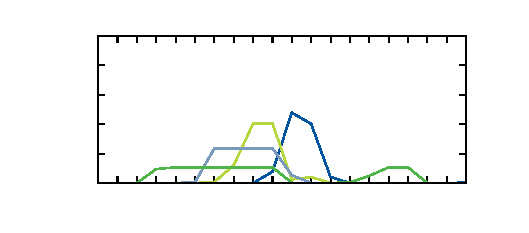
\includegraphics{GNUPlot/FB_converge}}%
    \gplfronttext
  \end{picture}%
\endgroup

        \caption{convergence failure.}
        \label{fig:conv_fail}
    \end{figure}

    This issue has been addressed, by \cite{Kraemer.2010} who propose a re-initialization strategy based on the magnitude of
    the Lagrange multipliers associated with the continuous variables. While the results using this adjusted strategy
    are very promising it could not be implemented within the scope of this thesis. In addition to the adjusted algorithm,
    the problem formulation can be altered to improve convergence of the solution algorithm. Two strategies can
    be employed, which exploit the structure of the distillation model, or force the continuous solution to both sides
    of the feasible domain \cite{Kraemer.2009}.

    The first strategy involves reformulation of purity constraints in terms of the reflux split
    \Eq{}{
        \sum_j \zeta_j^R x_j \leq x_{\text{spec}}.
    }
    As one will always observe a concentration gradient in a finite distillation column, this formulation favours
    integer solutions as it competes with a lower capital costs which distributes fractions on lower trays. Hence
    this strategy is assumed to be most successful for steep concentration gradients at either of the column.
    It should be considered, that this formulation requires the variable tray location to be on the side at which
    the specified purity lies. \todo{write about optimization model.}

    The second approach relies on the previously introduced differentiable distribution function. Here a sufficient
    focus on a given tray can be enforced by adjusting the underlying standard deviation. By introducing that function
    in the first optimization stage, while continuing with the traditional formulation in the subsequent steps,
    convergence could be achieved.

    \todo{discuss time consumption and quality of the solution.}

    \subsection{Steady state single period}
    \label{chp:optexample:ss_single_perid}
    Objective function
    \Eqml{eq:opt:ss_single_objective}{
        CAPEX = \left( \sum_c C_c^{\text{cap}} \right) \cdot \left(q^{-a} \frac{q^a - 1}{q - 1} \right) + \sum_o C_o^{\text{oper}} \\
            \eqannote{c = \left\{ \text{HPC}, \text{LPC}, \text{CAC}, \text{HX}, \text{CP}, \text{CRM}, \text{CRCAC} \right\}
                \quad o = \left\{\text{CP}, \text{EXP} \right\}}
    }
    Constraints :
    Limits on the product purities:
    \Eq{eq:opt:ss_single_constraints_1}{
        y_{1,N_2}^{HPC} & \geq 0.985 \\
        y_{1,N_2}^{LPC} & \geq 0.985 \\
        y_{1,Ar}^{CAC} & \geq 0.985 \\
        x_{reb}^{CRM} & \geq 0.985
    }
    No flooding in the columns:
    \Eq{eq:opt:ss_single_constraints_2}{
        d_{\text{column}}^{\text{HPC}} & \geq d_{min}^{HPC} \\
        d_{\text{column}}^{\text{LPC}} & \geq d_{min}^{LPC} \\
        d_{\text{column}}^{\text{CAC}} & \geq d_{min}^{CAC}
    }
    No entrainment in the trayed column :
    \Eq{eq:opt:ss_single_constraints_3}{
        \left(1- \sum_{k=1}^{j-1} \right) ent_k^{HPC} & \leq 0.1
    }
    Limit on cooling water outlet temperatures to prevent corrosion :
    \Eq{eq:opt:ss_single_constraints_4}{
        T_{\text{w,out}}^{IC1} & \leq 323.15 \\
        T_{\text{w,out}}^{IC2} & \leq 323.15 \\
        T_{\text{w,out}}^{IC3} & \leq 323.15
    }

    Design Variables
    \begin{itemize}
        \item HPC diameter $d_{\text{column}}^{\text{HPC}}$
        \item LPC diameter $d_{\text{column}}^{\text{LPC}}$
        \item CAC diameter $d_{\text{column}}^{\text{CAC}}$
        \item HPC reflux location $\zeta^R_{\text{HPC}}$
        \item LPC reflux location $\zeta^R_{\text{LPC}}$
        \item CAC reflux location $\zeta^R_{\text{CAC}}$
        \item LPC CAC side draw location $\zeta^{SV,\text{LPC}}_{2,j}$
        \item heat exchange area multi-stream heat exchanger $A_{\text{HX}}^{multiHX}$
        \item heat exchange area main condenser reboiler $A_{\text{HX}}^{CRM}$
        \item heat exchange area CAC condenser reboiler $A_{\text{HX}}^{CRCAC}$
    \end{itemize}

    Manipulated Variables
    \begin{itemize}
        \item intercooler outlet temperatures ($T_{\text{out}}^{IC1}, T_{\text{out}}^{IC2}, T_{\text{out}}^{IC3}$)
        \item HPC dimensionless side draw (gaseous $N_2$product) ($s_1^{V, \text{HPC}}$)
        \item LPC dimensionless side draws ($s_i^{V, \text{LPC}}$)
    \end{itemize}

\subsection{Optimization \& control}
	To include the design of a PI control structure in the process, the following constraints need to be added.
	\Eq{}{
		u_m & = b_{m,1} + \sum_{j=1}^{n_m} \left( K_{m,n} \cdot e_{m,n} + I_{m,n} \right),
			\eqannote{m = 1 \dots n_{in}}, \\
		e_{m,n} & = set_{m,n} - meas_{n} \eqannote{m = 1 \dots n_{in}, n = 1 \dots n_m}, \\
		\frac{\mathrm{d} I}{\mathrm{d} t} & = \frac{e_{m,n}}{\tau_{m.n}} \eqannote{m = 1
			\dots n_{in}, n = 1 \dots n_m}, \\
		\frac{\mathrm{d} I}{\mathrm{d} t} & = 0 \eqannote{m = 1 \dots n_{in}, n = 1 \dots n_m}, \\
		set_{m,n} & = set_{m-1,n} \eqannote{m = 2 \dots n_{in}, n = 1 \dots n_m}, \\
		K^L_{m,n} \cdot \zeta^C_{m,n} & \leq K_{m,n}  \leq K^U_{m,n} \eqannote{m = 1 \dots n_{in},
			n = 1 \dots n_m}, \\
		\sum_{m=1}^{n_m} \zeta_{m,n}^C & = 1 \eqannote{m = 1 \dots n_{in}}, \\
		\sum_{n=1}^{n_{in}} \zeta_{m,n}^C & = 1 \eqannote{n = 1 \dots n_{m}},
	}
	Since new states have been introduced, the corresponding initial conditions will have to be included
	\Eq{}{
		I_{m,n} (t = 0) & = 0, \eqannote{m = 1 \dots n_{in}, n = 1 \dots n_m} \\
		e_{m,n} (t = 0) & = 0, \eqannote{m = 1 \dots n_{in}, n = 1 \dots n_m} \\
	}
